\subsubsection{Verwendung}

\begin{figure}[ht]
  \begin{center}
  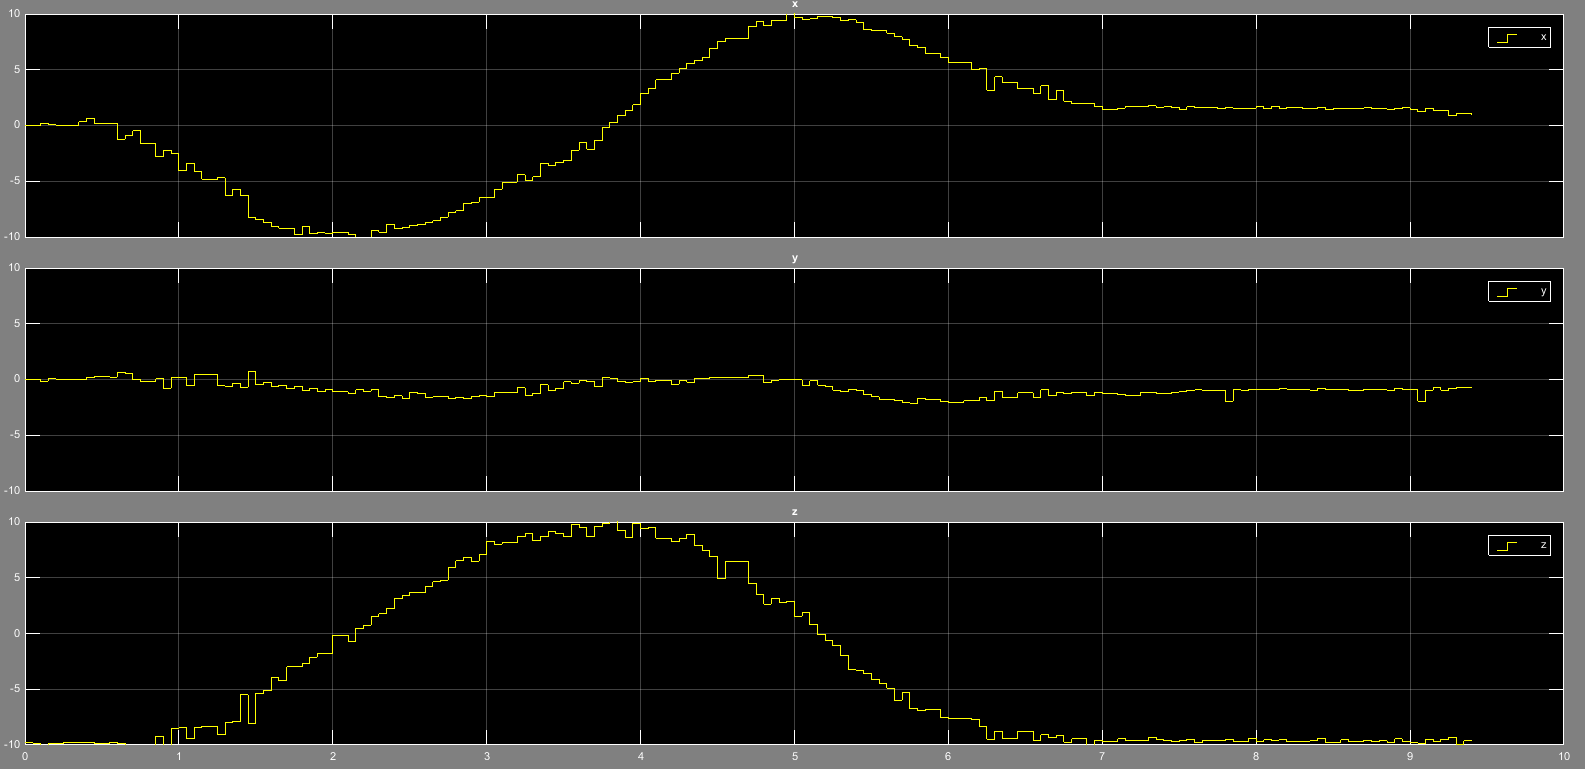
\includegraphics[scale=0.3]{pic/60_simulink/looping.png}
  \caption{Accelorometer während eines Looping}
  \label{fig:accel_looping}
  \end{center}
\end{figure}


\begin{figure}[ht]
  \begin{center}
  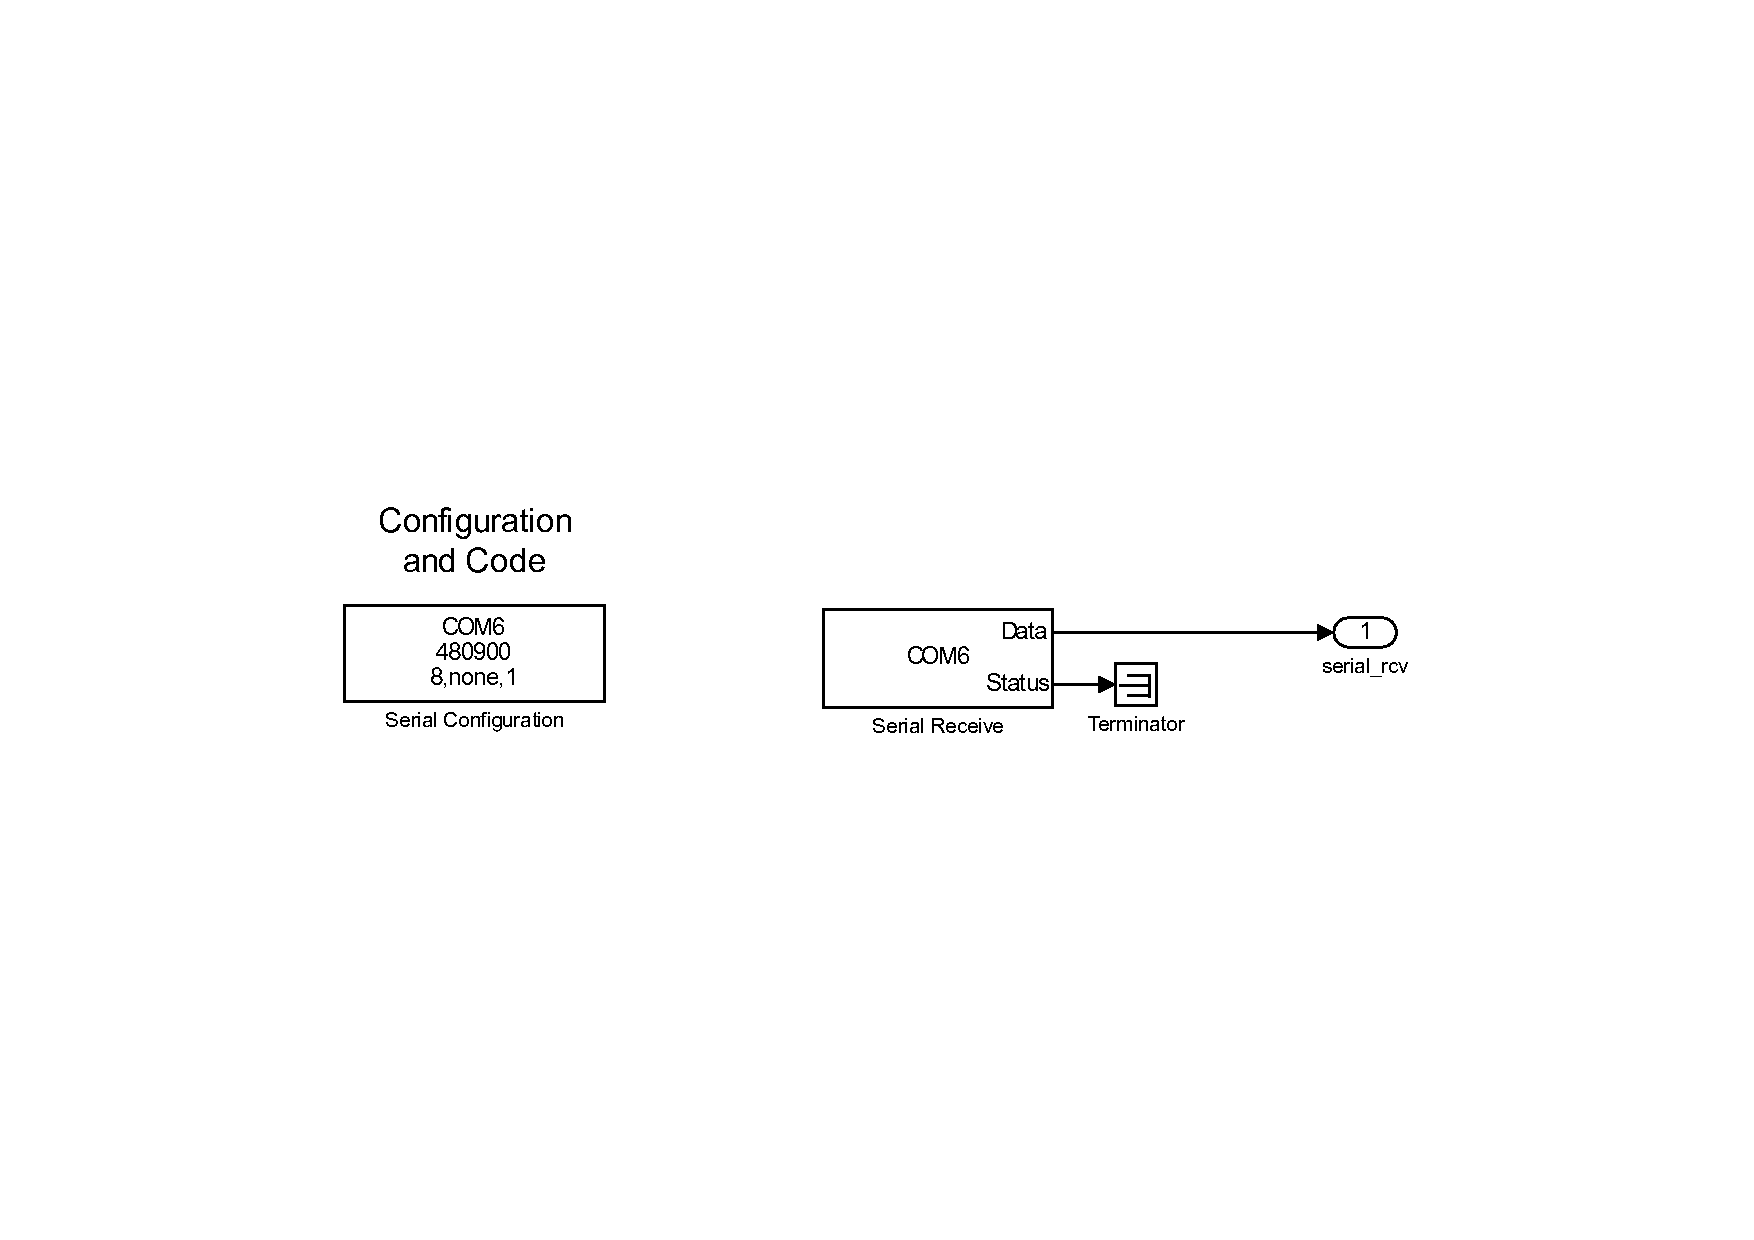
\includegraphics[scale=0.75, trim={5cm 8.5cm 6cm 8.5cm},clip]{pic/60_simulink/Serial_output.pdf}
  \caption{Serielle Schnittstelle}
  \label{fig:Serielle Schnittstelle}
  \end{center}
\end{figure}



\begin{figure}[ht]
  \begin{center}
  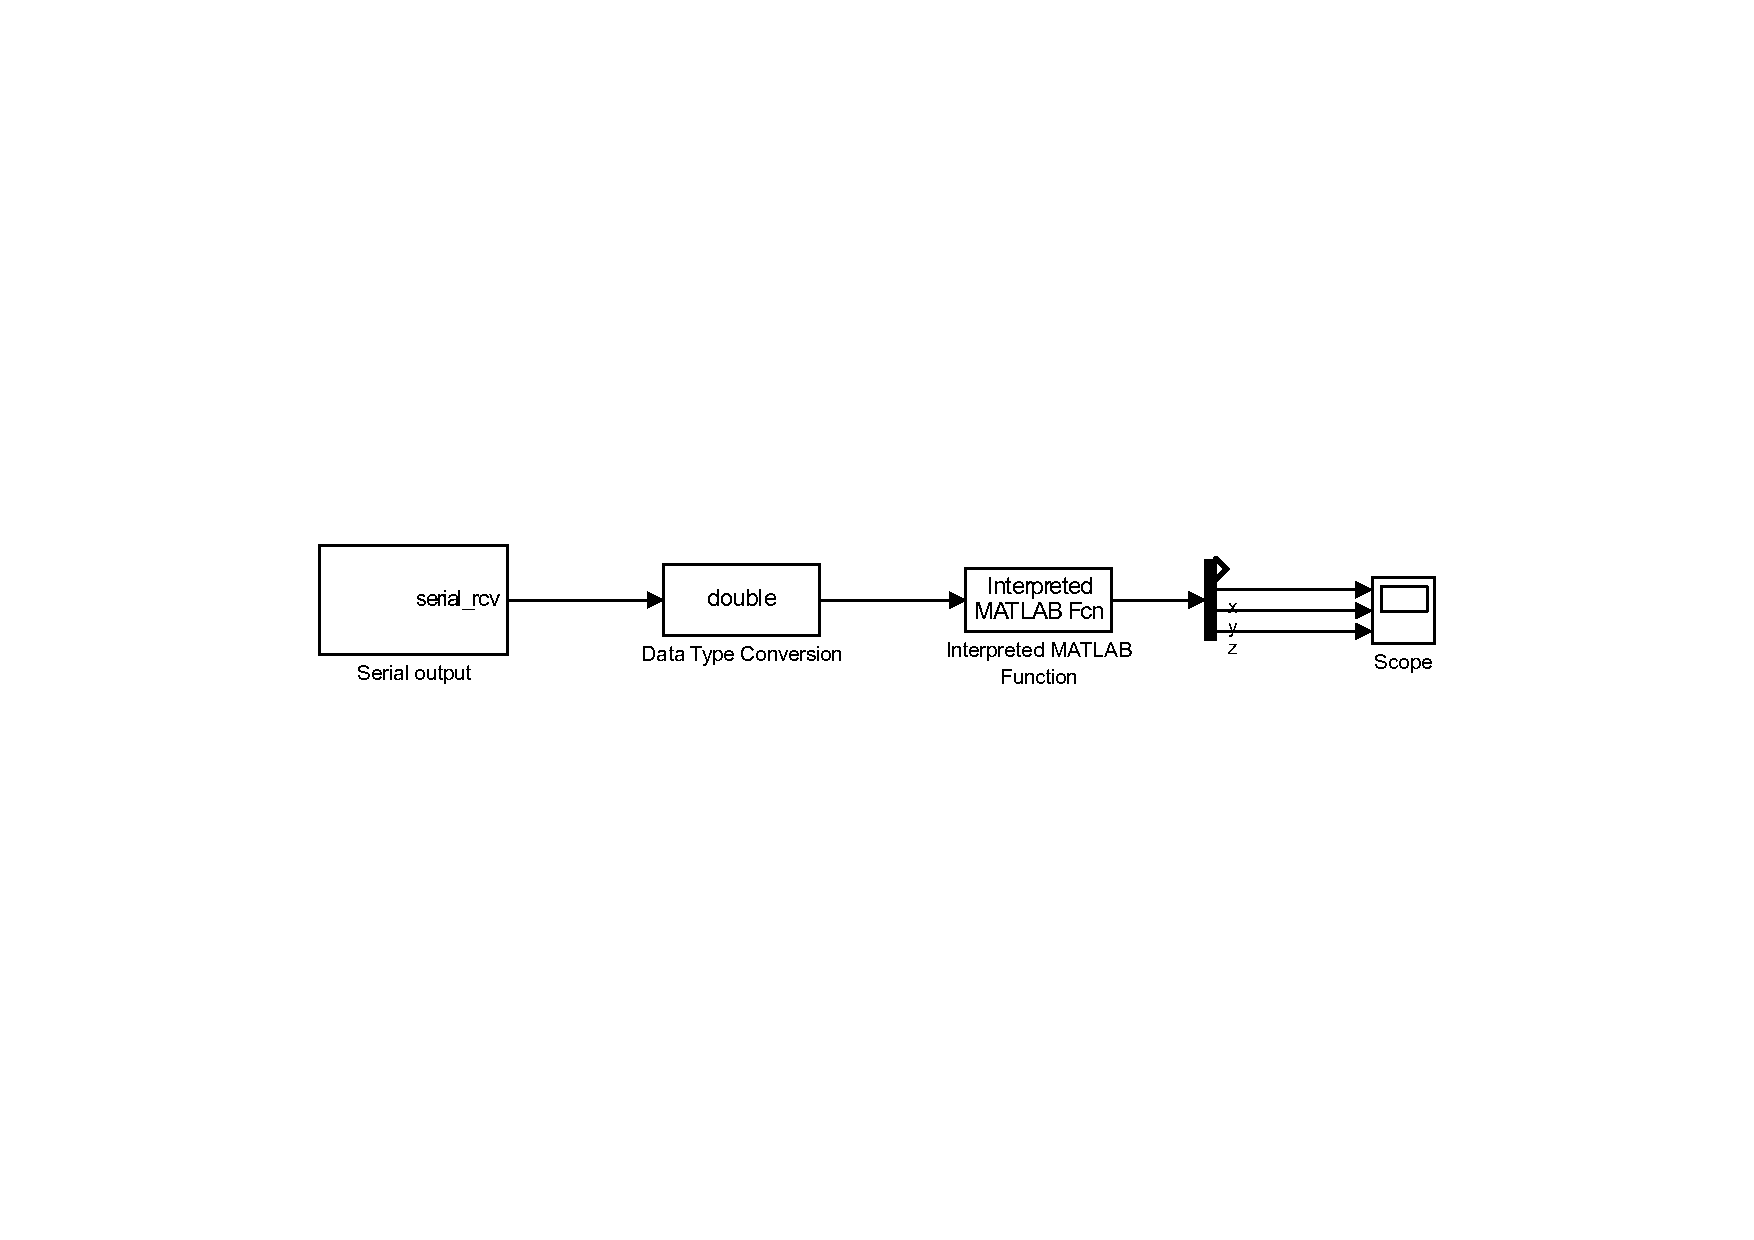
\includegraphics[scale=0.75, trim={5cm 9cm 4.8cm 8.5cm},clip]{pic/60_simulink/sys_main.pdf}
  \caption{Serielle Schnittstelle}
  \label{fig:Serielle Schnittstelle}
  \end{center}
\end{figure}



\clearpage
